\documentclass{article}

\usepackage[margin=0.8in]{geometry}
\usepackage{amsmath, amsfonts}
\usepackage{booktabs}
\usepackage{hyperref}
\usepackage{xcolor}
\usepackage{tikz}
\tikzset{block/.style ={rectangle,draw}
}
\usetikzlibrary{positioning, shapes.geometric}

\setlength{\parindent}{0pt}

\begin{document}

\section*{EVB Decomposition}
Change in the value function due to learning after taking action $a^*$:

\begin{align}
v(ba^*)-v(b)=&\sum_{b'}p(b'\mid b, a^*)\Big(v(b')-v(b)\Big)\\
=&\sum_{b'}p(b'\mid b, a^*)\Big(\sum_a \pi(a\mid b')q(b', a)-\sum_{a} \pi(a\mid b)q(b,a)\Big) \nonumber \\
=&\sum_{b'}p(b'\mid b, a^*)\sum_a\Big(\big(\pi(a\mid b')-\pi(a\mid b)\big)q(b',a) \nonumber \\
+&\pi(a\mid b)\big(q(b', a) - q(b, a)\big)\Big) \nonumber
\end{align}

Expanding $q(b', a) - q(b, a)$:

\begin{align}
q(b', a)-q(b, a)=&\sum_{b''}p(b''\mid b', a)\big[r(b',a) + \gamma v(b'')\big]\\
-&\sum_{b'}p(g'\mid b, a)\big[r(b,a) + \gamma v(g')\big]\nonumber\\
=& r(b',a) + \gamma \sum_{b''}p(b''\mid b', a)v(b'')\nonumber \\
-& r(b,a) + \gamma \sum_{g'}p(g'\mid b, a)v(g')\nonumber \\
=& \underbrace{\vphantom{ \left(\frac{a^{\frac{0.3}{`}}}{b}\right)} r(b',a) - r(b,a)}_{\substack{\text{Difference in the expected} \\ \text{immediate return}}} + \underbrace{\gamma \big[ \sum_{b''}p(b''\mid b', a)v(b'') - \sum_{g'}p(g'\mid b, a)v(g') \big]}_{\substack{\text{Difference in the expected} \\ \text{future return}}}\nonumber
\end{align}

So overall the EVB decomposes as:

\begin{align}
    v(ba^*)-v(b) =& \mathbb{E}_{b'\sim p(b'\mid b, a^*)}\Big[\sum_a \big(\pi(a\mid b')-\pi(a\mid b)\big)q(b',a) \\
    +& \mathbb{E}_{a\sim \pi(a\mid b)}\big[r(b',a) - r(b,a)\big] \nonumber \\ 
    +& \mathbb{E}_{a\sim \pi(a\mid b)}\big[\gamma \sum_{b''}p(b''\mid b', a)v(b'') - \gamma \sum_{g'}p(g'\mid b, a)v(g') \big] \Big] \nonumber
\end{align}

One last thing to consider is how the prioritisation of distal experiences should 
differ from those that are more immediate. This also has implications for how likely 
those experiences are to occur according to the current model. 
\bigbreak
For instance, if the agent considers updating $v(b)$ towards the value that would result 
from taking a particular action from that belief state -- say, $v(ba^*)$ -- the EVB associated 
with that update needs to be weighted by the probability of transitioning into 
belief state $b$ in the first place (i.e., from the current root of the tree).

\begin{align}
    v(ba^*)-v(b) = p(b_{\text{root}}\rightarrow b) &\mathbb{E}_{b'\sim p(b'\mid b, a^*)}\Big[\sum_a \big(\pi(a\mid b')-\pi(a\mid b)\big)q(b',a) \\
    +& \mathbb{E}_{a\sim \pi(a\mid b)}\big[r(b',a) - r(b,a)\big] \nonumber \\ 
    +& \mathbb{E}_{a\sim \pi(a\mid b)}\big[\gamma \sum_{b''}p(b''\mid b', a)v(b'') - \gamma \sum_{g'}p(g'\mid b, a)v(g') \big] \Big] \nonumber
\end{align}

\newpage
\section*{Simulations}

Prioritisation pattern with horizon $h=2$.
\vspace{1cm}

\begin{minipage}{\textwidth}
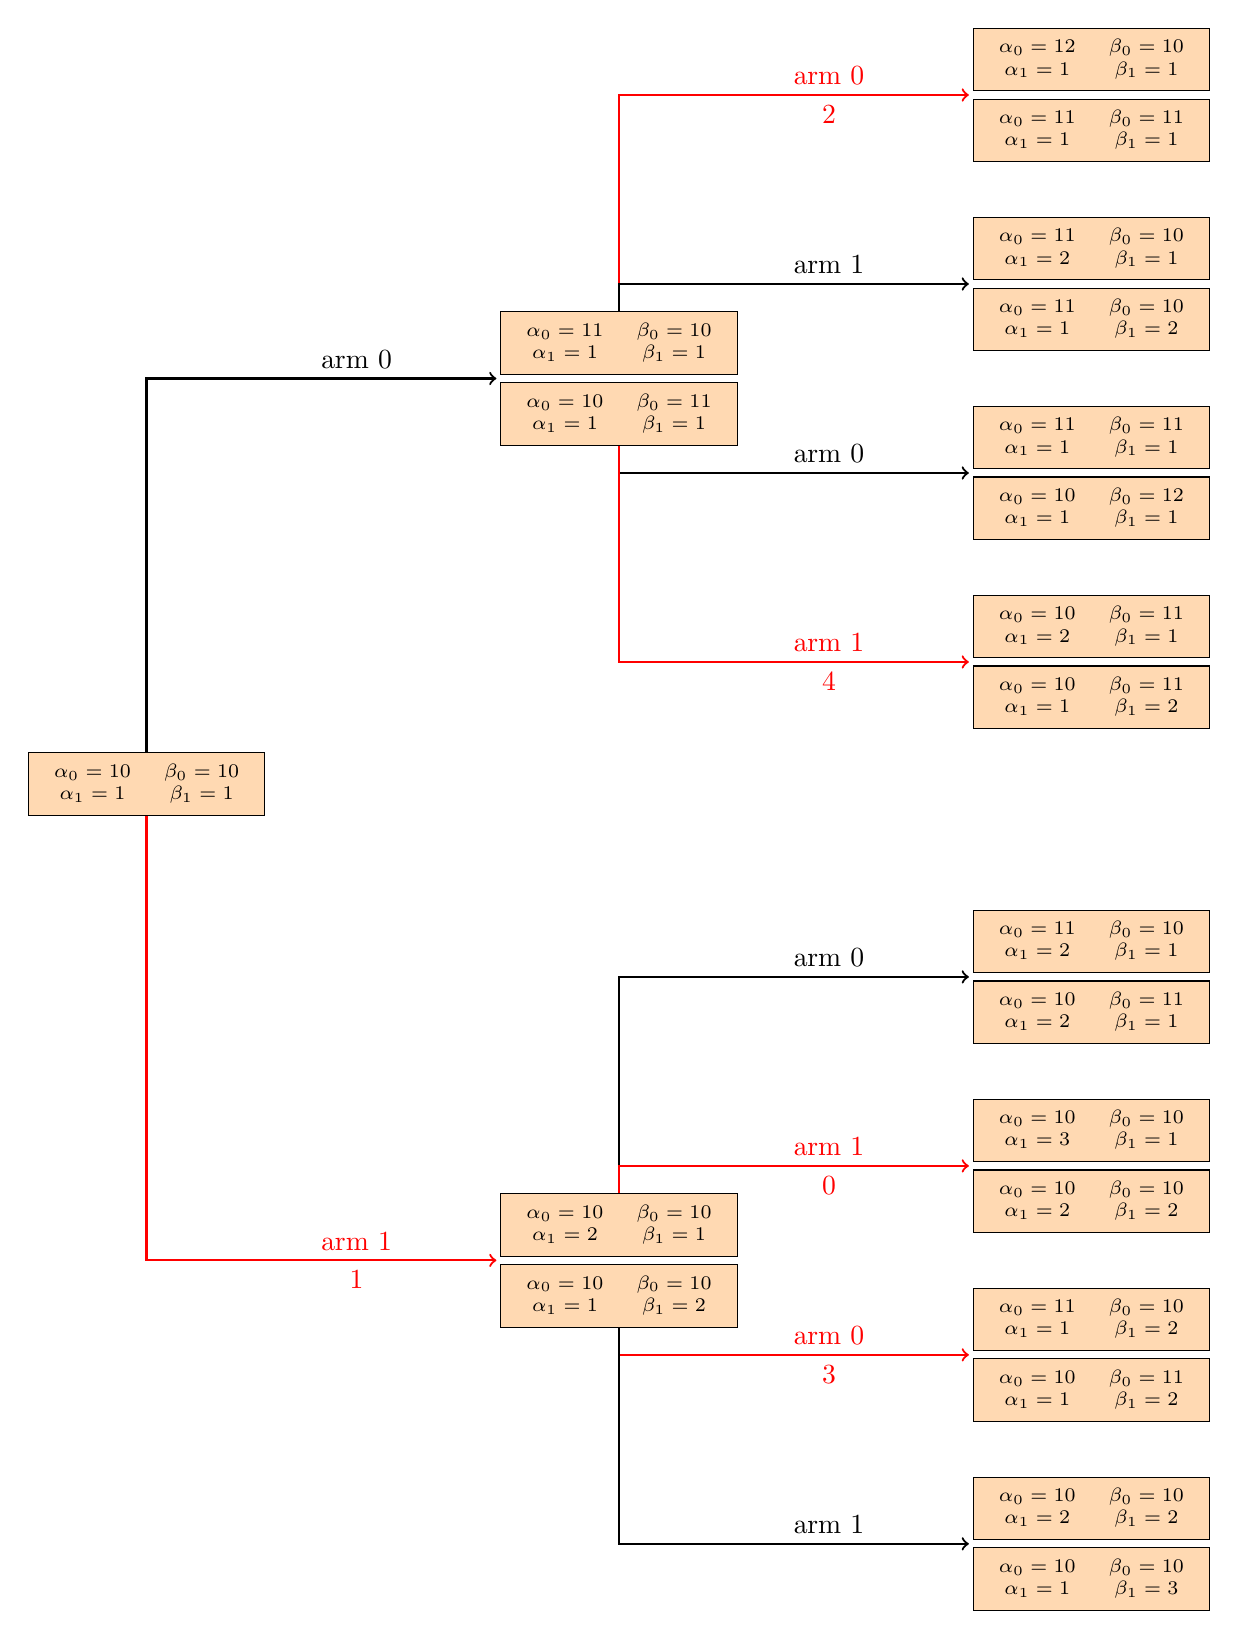
\begin{tikzpicture}
\tikzstyle{state}   = [rectangle, text centered, draw=black, minimum width=2.2cm, fill=orange!30]
\tikzstyle{between} = [rectangle, draw=none, minimum width=3.1cm]
\node[state] at (-8.00, 0.00)   (h0){\scriptsize \begin{tabular}{c c} $\alpha_0=10$ & $\beta_0=10$ \\ $\alpha_1=1$ & $\beta_1=1$ \end{tabular}};
\node[state] at (-2.00, 5.60)  (h1_0){\scriptsize \begin{tabular}{c c} $\alpha_0=11$ & $\beta_0=10$ \\ $\alpha_1=1$ & $\beta_1=1$ \end{tabular}};
\node[between] at (-2.00, 5.15) (h1_01){};
\node[state] at (-2.00, 4.70)(h1_1){\scriptsize \begin{tabular}{c c} $\alpha_0=10$ & $\beta_0=11$ \\ $\alpha_1=1$ & $\beta_1=1$ \end{tabular}};
\node[state] at (-2.00, -5.60)  (h1_2){\scriptsize \begin{tabular}{c c} $\alpha_0=10$ & $\beta_0=10$ \\ $\alpha_1=2$ & $\beta_1=1$ \end{tabular}};
\node[between] at (-2.00, -6.05) (h1_23){};
\node[state] at (-2.00, -6.50)(h1_3){\scriptsize \begin{tabular}{c c} $\alpha_0=10$ & $\beta_0=10$ \\ $\alpha_1=1$ & $\beta_1=2$ \end{tabular}};
\node[state] at (4.00, 9.20)  (h2_0){\scriptsize \begin{tabular}{c c} $\alpha_0=12$ & $\beta_0=10$ \\ $\alpha_1=1$ & $\beta_1=1$ \end{tabular}};
\node[between] at (4.00, 8.75) (h2_01){};
\node[state] at (4.00, 8.30)(h2_1){\scriptsize \begin{tabular}{c c} $\alpha_0=11$ & $\beta_0=11$ \\ $\alpha_1=1$ & $\beta_1=1$ \end{tabular}};
\node[state] at (4.00, 6.80)  (h2_2){\scriptsize \begin{tabular}{c c} $\alpha_0=11$ & $\beta_0=10$ \\ $\alpha_1=2$ & $\beta_1=1$ \end{tabular}};
\node[between] at (4.00, 6.35) (h2_23){};
\node[state] at (4.00, 5.90)(h2_3){\scriptsize \begin{tabular}{c c} $\alpha_0=11$ & $\beta_0=10$ \\ $\alpha_1=1$ & $\beta_1=2$ \end{tabular}};
\node[state] at (4.00, 4.40)  (h2_4){\scriptsize \begin{tabular}{c c} $\alpha_0=11$ & $\beta_0=11$ \\ $\alpha_1=1$ & $\beta_1=1$ \end{tabular}};
\node[between] at (4.00, 3.95) (h2_45){};
\node[state] at (4.00, 3.50)(h2_5){\scriptsize \begin{tabular}{c c} $\alpha_0=10$ & $\beta_0=12$ \\ $\alpha_1=1$ & $\beta_1=1$ \end{tabular}};
\node[state] at (4.00, 2.00)  (h2_6){\scriptsize \begin{tabular}{c c} $\alpha_0=10$ & $\beta_0=11$ \\ $\alpha_1=2$ & $\beta_1=1$ \end{tabular}};
\node[between] at (4.00, 1.55) (h2_67){};
\node[state] at (4.00, 1.10)(h2_7){\scriptsize \begin{tabular}{c c} $\alpha_0=10$ & $\beta_0=11$ \\ $\alpha_1=1$ & $\beta_1=2$ \end{tabular}};
\node[state] at (4.00, -2.00)  (h2_8){\scriptsize \begin{tabular}{c c} $\alpha_0=11$ & $\beta_0=10$ \\ $\alpha_1=2$ & $\beta_1=1$ \end{tabular}};
\node[between] at (4.00, -2.45) (h2_89){};
\node[state] at (4.00, -2.90)(h2_9){\scriptsize \begin{tabular}{c c} $\alpha_0=10$ & $\beta_0=11$ \\ $\alpha_1=2$ & $\beta_1=1$ \end{tabular}};
\node[state] at (4.00, -4.40)(h2_10){\scriptsize \begin{tabular}{c c} $\alpha_0=10$ & $\beta_0=10$ \\ $\alpha_1=3$ & $\beta_1=1$ \end{tabular}};
\node[between] at (4.00, -4.85) (h2_1011){};
\node[state] at (4.00, -5.30)(h2_11){\scriptsize \begin{tabular}{c c} $\alpha_0=10$ & $\beta_0=10$ \\ $\alpha_1=2$ & $\beta_1=2$ \end{tabular}};
\node[state] at (4.00, -6.80)(h2_12){\scriptsize \begin{tabular}{c c} $\alpha_0=11$ & $\beta_0=10$ \\ $\alpha_1=1$ & $\beta_1=2$ \end{tabular}};
\node[between] at (4.00, -7.25) (h2_1213){};
\node[state] at (4.00, -7.70)(h2_13){\scriptsize \begin{tabular}{c c} $\alpha_0=10$ & $\beta_0=11$ \\ $\alpha_1=1$ & $\beta_1=2$ \end{tabular}};
\node[state] at (4.00, -9.20)(h2_14){\scriptsize \begin{tabular}{c c} $\alpha_0=10$ & $\beta_0=10$ \\ $\alpha_1=2$ & $\beta_1=2$ \end{tabular}};
\node[between] at (4.00, -9.65) (h2_1415){};
\node[state] at (4.00, -10.10)(h2_15){\scriptsize \begin{tabular}{c c} $\alpha_0=10$ & $\beta_0=10$ \\ $\alpha_1=1$ & $\beta_1=3$ \end{tabular}};
\draw[->, thick, black] ([yshift=5.5cm]h0)   |- (h1_01)  node[above, pos=0.8] {arm $0$} node[below, pos=0.8] {};
\draw[->, thick, red] ([yshift=-5.5cm]h0)  |- (h1_23)  node[above, pos=0.8] {arm $1$} node[below, pos=0.8] {1};
\draw[->, thick, red] ([yshift=4.0cm]h1_0) |- (h2_01)  node[above, pos=0.8] {arm $0$} node[below, pos=0.8] {2};
\draw[->, thick, black] ([yshift=1.5cm]h1_0) |- (h2_23)  node[above, pos=0.8] {arm $1$} node[below, pos=0.8] {};
\draw[->, thick, black] ([yshift=1.5cm]h1_1) |- (h2_45)  node[above, pos=0.8] {arm $0$} node[below, pos=0.8] {};
\draw[->, thick, red] ([yshift=1.5cm]h1_1) |- (h2_67)  node[above, pos=0.8] {arm $1$} node[below, pos=0.8] {4};
\draw[->, thick, black] ([yshift=1.5cm]h1_2) |- (h2_89)  node[above, pos=0.8] {arm $0$} node[below, pos=0.8] {};
\draw[->, thick, red] ([yshift=1.5cm]h1_2) |- (h2_1011) node[above, pos=0.8] {arm $1$} node[below, pos=0.8] {0};
\draw[->, thick, red] ([yshift=1.5cm]h1_3) |- (h2_1213) node[above, pos=0.8] {arm $0$} node[below, pos=0.8] {3};
\draw[->, thick, black] ([yshift=1.5cm]h1_3) |- (h2_1415) node[above, pos=0.8] {arm $1$} node[below, pos=0.8] {};
\end{tikzpicture}
\end{minipage}


\end{document}
